% !TEX TS-program = pdflatexmk
\documentclass[12pt]{amsart}
\usepackage{amsmath}
\usepackage{amssymb}
\usepackage{xcolor}
\definecolor{dark-red}{rgb}{0.7,0.25,0.25}
\definecolor{dark-blue}{rgb}{0.15,0.15,0.55}
\definecolor{medium-blue}{rgb}{0,0,0.65}

\usepackage{tikz}
\usetikzlibrary{cd}
\usetikzlibrary{knots}
\usetikzlibrary{calc}

\usepackage{graphicx}
\usepackage{fullpage}
\usepackage[T1]{fontenc}
\usepackage[final]{microtype}
\usepackage{libertine}
\usepackage[libertine]{newtxmath}
\usepackage{ifthen}

\usepackage[pdftex,plainpages=false,hypertexnames=false,pdfpagelabels,breaklinks]{hyperref}
\hypersetup{
   colorlinks, linkcolor={purple},
   citecolor={medium-blue}, urlcolor={medium-blue}
}
\urlstyle{same}

\newcommand{\arxiv}[1]{\href{https://arxiv.org/abs/#1}{\small  arXiv:#1}}

\newcommand{\nn}[1]{{\color{red} [[#1]]}}

% tricky way to iterate macros over a list
\def\semicolon{;}
\def\applytolist#1{
    \expandafter\def\csname multi#1\endcsname##1{
        \def\multiack{##1}\ifx\multiack\semicolon
            \def\next{\relax}
        \else
            \csname #1\endcsname{##1}
            \def\next{\csname multi#1\endcsname}
        \fi
        \next}
    \csname multi#1\endcsname}

% \def\cA{{\cal A}} for A..Z
\def\calc#1{\expandafter\def\csname c#1\endcsname{{\mathcal #1}}}
\applytolist{calc}QWERTYUIOPLKJHGFDSAZXCVBNM;
% \def\bbA{{\mathbb A}} for A..Z
\def\bbc#1{\expandafter\def\csname bb#1\endcsname{{\mathbb #1}}}
\applytolist{bbc}QWERTYUIOPLKJHGFDSAZXCVBNM;
% \def\bfA{{\mathbf A}} for A..Z
\def\bfc#1{\expandafter\def\csname bf#1\endcsname{{\mathbf #1}}}
\applytolist{bfc}QWERTYUIOPLKJHGFDSAZXCVBNM;

\newcommand{\Kar}{\operatorname{Kar}}
\newcommand{\Obj}{\operatorname{Obj}}
\newcommand{\Fun}{\operatorname{Fun}}
\newcommand{\Set}{\mathsf{Set}}
\renewcommand{\Vec}{\mathsf{Vec}}
\newcommand{\fdVec}{\mathsf{fdVec}}
\newcommand{\Rep}{\mathsf{Rep}}

\begin{document}

\title{Problems for the category theory reading course, 2017}
\author{Scott Morrison}
  \address[Scott Morrison]{
  	Mathematical Sciences Institute,
  	Australian National University
  }
  \email{\href{mailto:scott.morrison@anu.edu.au}{scott.morrison@anu.edu.au}}
\date{Version of \today}

\maketitle

\section{Assignment 1, due end of Week 4}

\subsection{Functors}
\begin{enumerate}
\item Leinster 1.2.21 (functors preserve isomorphisms)
\item Leinster 1.2.27, 1.2.28b (full, faithful)
\end{enumerate}

\subsection{Natural transformations}
\begin{enumerate}
\item In $\sf{fdVec}$, show that the functors $\operatorname{id}$ and $**$ are naturally isomorphic. 
\item Show the the vertical composition of two natural transformations is in fact a natural transformation.
\item Prove carefully that the horizontal composition of two natural transformations is again a natural transformation.
\item Show that a functor $F : \cC \to \cD$ is part of an equivalence of categories if and only if it is \emph{fully faithful} and \emph{essentially surjective}. Clearly state where you are using the axiom of choice, or add hypotheses so it is unnecessary.
\end{enumerate}

\subsection{Universal properties}
\begin{enumerate}
\item Prove that two initial objects in a category are isomorphic.
\item For each of the following categories, decide whether there is an initial, final, and/or zero object, and if so, describe them:
$\sf{FinSet}$, $\sf{fdVec}$, $\sf{Top}$, $\sf{Top}_*$ (pointed topological spaces), field extensions of a fixed field $F$, $\sf{Graphs}$ (your answer may depend on which class of graphs you consider), $\sf{Semigroups}$, $\sf{Groups}$.
\item Describe the product of two objects as the terminal object in some category.
\item Describe the tensor product of two vectors spaces as the initial object in some category.
\item Describe both the product and coproduct in the following categories: $\sf{FinSet}$, $\sf{Top}$, $\sf{Top}_*$, $\sf{AbGroup}$, $\sf{Group}$, $\sf{Graphs}$.
\end{enumerate}


% \section{Equivalences}
% \begin{enumerate}
% \item Choose one of the following pairs of categories, and carefully show that they are equivalent:
% \begin{itemize}
% 	\item Compact Hausdorff topological spaces, and commutative $C^*$-algebras.
% 	\item Subgroups of $\pi_1(X)$, and covers of $X$. (A condition is needed on $X$ to make this work. What is it?)
% 	\item Subgroups of $\operatorname{Gal}(E \subset F)$, and intermediate field extensions. (A condition is needed on $E \subset F$ to make this work. What is it?)
% \end{itemize}
% \end{enumerate}

\subsection{Adjunctions}
\begin{enumerate}
\item Consider the forgetful functor from abelian groups to groups. What is its left adjoint?
\item In the category of finite dimensional vector spaces, show that $- \otimes V$ is biadjoint to $- \otimes V^*$.
\item Prove that the `hom-set isomorphism' and `unit/counit' definitions of an adjunction are equivalent.
\end{enumerate}
% \item Consider the functors
% \begin{align*}
% gr : & \operatorname{filVec} \to \operatorname{grVec} \\
%      & ( \cdots \subset V_i \subset V_{i+1} \subset \cdots ) \mapsto \bigoplus_i V_{i+1} / V_i \\
% \intertext{and}
% fil : & \operatorname{filVec} \to \operatorname{grVec} \\
%       & \bigoplus_i V_i \mapsto (\cdots \subset \bigoplus_{j\leq i} V_j \subset \bigoplus_{j\leq i+1} V_j \subset \cdots). 
% \end{align*}
% Describe the left and right adjoints, if they exist.


\section{Assignment 2, due at the end of Week 7:}
\subsection{Idempotent completion}
The `idempotent completion' $\Kar(\cC)$ (also called the `Karoubi envelope') is defined as follows:
\begin{align*}
\Obj \Kar(\cC) & = \left\{ (X \in \Obj(\cC), p :  X \to X) \mid| p^2 = p \right\} \\
\Kar(\cC)((X,p) \to (X',p')) & = \left\{ f \in \cC(X \to X') \mid| fp = f = p'f \right\}.
\end{align*}
\begin{enumerate}
\item Let $\mathsf{primeVec}$ denote the full subcategory of $\mathsf{Vec}$ consisting of vector spaces with prime dimensions. Show carefully that $\Kar(\mathsf{primeVec}) \cong \mathsf{Vec}$.
\item Construct an equivalence $\iota_\cC : \Kar(\Kar(\cC)) \cong \Kar(\cC)$.
\item Show that there is a fully faithful functor $\cC \to \Kar(\cC)$ given by $X \mapsto (X, 1_X)$.
\item Note that given a functor $F : \cC \to \cD$, there is functor $\Kar(F) : \Kar(\cC) \to \Kar(\cD)$ given by
\begin{align*}
\Kar(F)(X,p) & = (F(X), F(p)) \\
\Kar(F)(f : (X,p) \to (X',p')) & = F(f).
\end{align*}
(You might say that $\Kar$ is a 2-functor from $\mathsf{CAT}$ to itself --- what does this mean at the level of natural transformations?)
Given a functor $F : \Kar(C) \to \Kar(D)$, show that it is determined up to natural isomorphism by its restriction $F|_\cC : C \to \Kar(D)$, by showing $F \cong (\iota_\cD \circ \Kar(F|_\cC))$.
\item (Not on the problem set: there is a forgetful 2-functor $\mathsf{CAT} \to \mathsf{SemiCat}$, the 2-category of `semicategories' (categories without identities) and their functors and natural transformations. The idempotent completion gives a 2-functor $\mathsf{SemiCAT} \to \mathsf{CAT}$. Are they an adjoint pair?)
\end{enumerate}

\subsection{Limits}
\begin{enumerate}
\item
Recall that given a functor $F : \cJ \to \cC$, the \emph{limit} of $F$, written $\lim_\cJ F$ is a terminal object in the category of cones over $F$. Explicitly, a cone consists of
\begin{enumerate}
	\item an object $X \in \Obj\cC$,
	\item for each $j \in \Obj\cC$, a map $f_j : X \to F(j)$,
	\item such that for any $g:j \to j'$, $F(g) \circ f_j = f_{j'}$.
\end{enumerate}
Another way of saying this is that the category of cones is the comma category $(J \downarrow F)$, where here we interpret $\cJ$ as a functor $\cC \to \Fun(\cJ \to \cC)$ by $c \mapsto (j \mapsto c)$ and we interpret $F$ as a functor $1 \to \Fun(\cJ \to \cC)$ by $1 \mapsto (j \mapsto F(j))$. Explain carefully why these are talking about the same thing!
\end{enumerate}


\subsection{The Yoneda embedding}
\begin{enumerate}
\item Prove the Yoneda lemma.
\item Explain why $\Fun(\cC^\text{op} \to \cD) = \Fun(\cC \to \cD^\text{op})$. Prove that $\Set^\text{op} \ncong \Set$, but that $\fdVec^\text{op} \cong \fdVec$.
\end{enumerate}

\newpage
\section{Assignment 3, due May 12:}
\begin{enumerate}
\item Prove that every monoidal category is monoidally equivalent to a strict monoidal category.

(Hint: given a monoidal category $\cC$, define a new monoidal category $\mathsf{List} \cC$, whose objects are lists of objects in $\cC$. In $\mathsf{List} \cC$, tensor product of objects is concatenation of lists, and the tensor unit is the empty list. There should be a functor $\mathsf{List} \cC$ to $\cC$ defined by sending a list to the tensor product of the elements of that list. Your job is to describe what happens at the level of morphisms, and check that everything works.)

\item Find an example of a monoidal functor which is not naturally isomorphic to any strict monoidal functor.

(Hint: consider categories $\Vec^\omega G$, where $G$ is a finite group, and $\omega \in H^3(G, k^\times)$ is a 3-cocycle. In particular, consider $G = \mathbb Z / 2 \mathbb Z$. The category $\Vec \mathbb Z / 2 \mathbb Z$ can be made into a monoidal category in two
distinct ways: either with the `obvious' associator, or with the associator $\alpha_{X, Y, Z} : (X \otimes Y) \otimes Z \to X \otimes (Y \otimes Z)$ which, when $Z$ is 1-dimensional, is either the identity if $Z$ is in the even grading, or minus the identity if $Z$ is in the odd grading. If you're going to use this example you should explain carefully why this associator works. You should be able to show that there are \emph{no} strict monoidal functors between these two versions of $\Vec \mathbb Z / 2 \mathbb Z$, but nevertheless there are non-strict monoidal functors, with a non-trivial tensorator; you should write one down explicitly.)

\item Let $\cC$ be a monoidal category. We say a `monoid object' in $\cC$ (or, as we gain confidence, just a monoid in $\cC$) is a tuple $(A \in \Obj C, \iota: 1 \to A, m: A \otimes A \to A)$ satisfying some conditions. Look up, or work out, what these conditions should be. (Hint: look at chapter 7 of Etingof, Gelaki, Nikshych, and Ostrik's book \href{http://www-math.mit.edu/~etingof/egnobookfinal.pdf}{Tensor Categories}.) You should be able to show that a monoid object in $\mathsf{Vec}$ is what is usually called an associative unital algebra.
\begin{enumerate}
\item A `module object' for a monoid object $A \in \cC$ is a tuple $(M, \triangleright: A \otimes M \to M)$ satisfying an appropriate condition (what is it?). A morphism $f$ between module objects $M$ and $M'$ is a morphism between the underlying objects, such that $f \circ \triangleright_M = \triangleright_{M'} \circ (1_A \otimes f)$. Draw the string diagram corresponding to this axiom. Define composition of module morphisms, by imitating the definition for modules over a ring. Show that modules for a fixed monoid object form a category.
\end{enumerate}
\item Show that $\Rep G$, for $G$ a finite group, forms a monoidal category.
\item If $\Rep G \cong \Rep H$, as categories, are $G$ and $H$ isomorphic? (Hint: no, give a counterexample.) What about if $\Rep G \cong \Rep H$ as monoidal categories, and moreover this equivalence is compatible with the forgetful functors to $\Vec$? (Hint: think about the monoidal automorphisms of the forgetful functor.) What if we drop the condition about compatibility with the forgetful functors? (Hint: google `isocategorical group'; you can answer this with just an appropriate reference to the literature, or do it yourself.)
\end{enumerate}

\newpage
\section{Assignment 4, due May 26:}
\subsection{Abelian categories}
\begin{enumerate}
\item Show if $F:\cC\to\cD$ is a fully faithful functor, then $f \in \cC(X \to Y)$ is a monomorphism if and only if $F(f)$ is. (Similarly for epimorphisms.)
\item Use this, and the Yoneda embedding, to show that in a rigid abelian category, the functor $- \otimes X$ is exact. (See Proposition 2.1.8 of Bakalov-Kirillov, attached, if you need some help; they don't explain how they are using Yoneda, however! You may cite the literature for any lemmas you like.)
\end{enumerate}

\subsection{Braided monoidal categories}
\begin{enumerate}
\item Explain how any object $X$ in a pivotal braided category gives an oriented link invariant.
\item Describe how the Temperley-Lieb category has the structure of a pivotal braided category.
\item Calculate the invariant of the trefoil corresponding to the object $1$ in Temperley-Lieb. (What is this invariant usually called?)
\item Show that in $\Kar(TL)$, we have $(2,1_2) \cong (2,f^{(2)}) \oplus (0, 1_0)$. (Here $f^{(2)}$ denotes the second Jones-Wenzl idempotent.)
\item Calculate the invariant of the unknot corresponding to the object $(2,f^{(2)})$ in (the idempotent completion of) Temperley-Lieb.
\item We say a monoid $(A, m)$ in a braided monoidal category is commutative if $m \circ \beta = m$. Define a monoidal structure on the category of modules for a commutative monoid.
\end{enumerate}

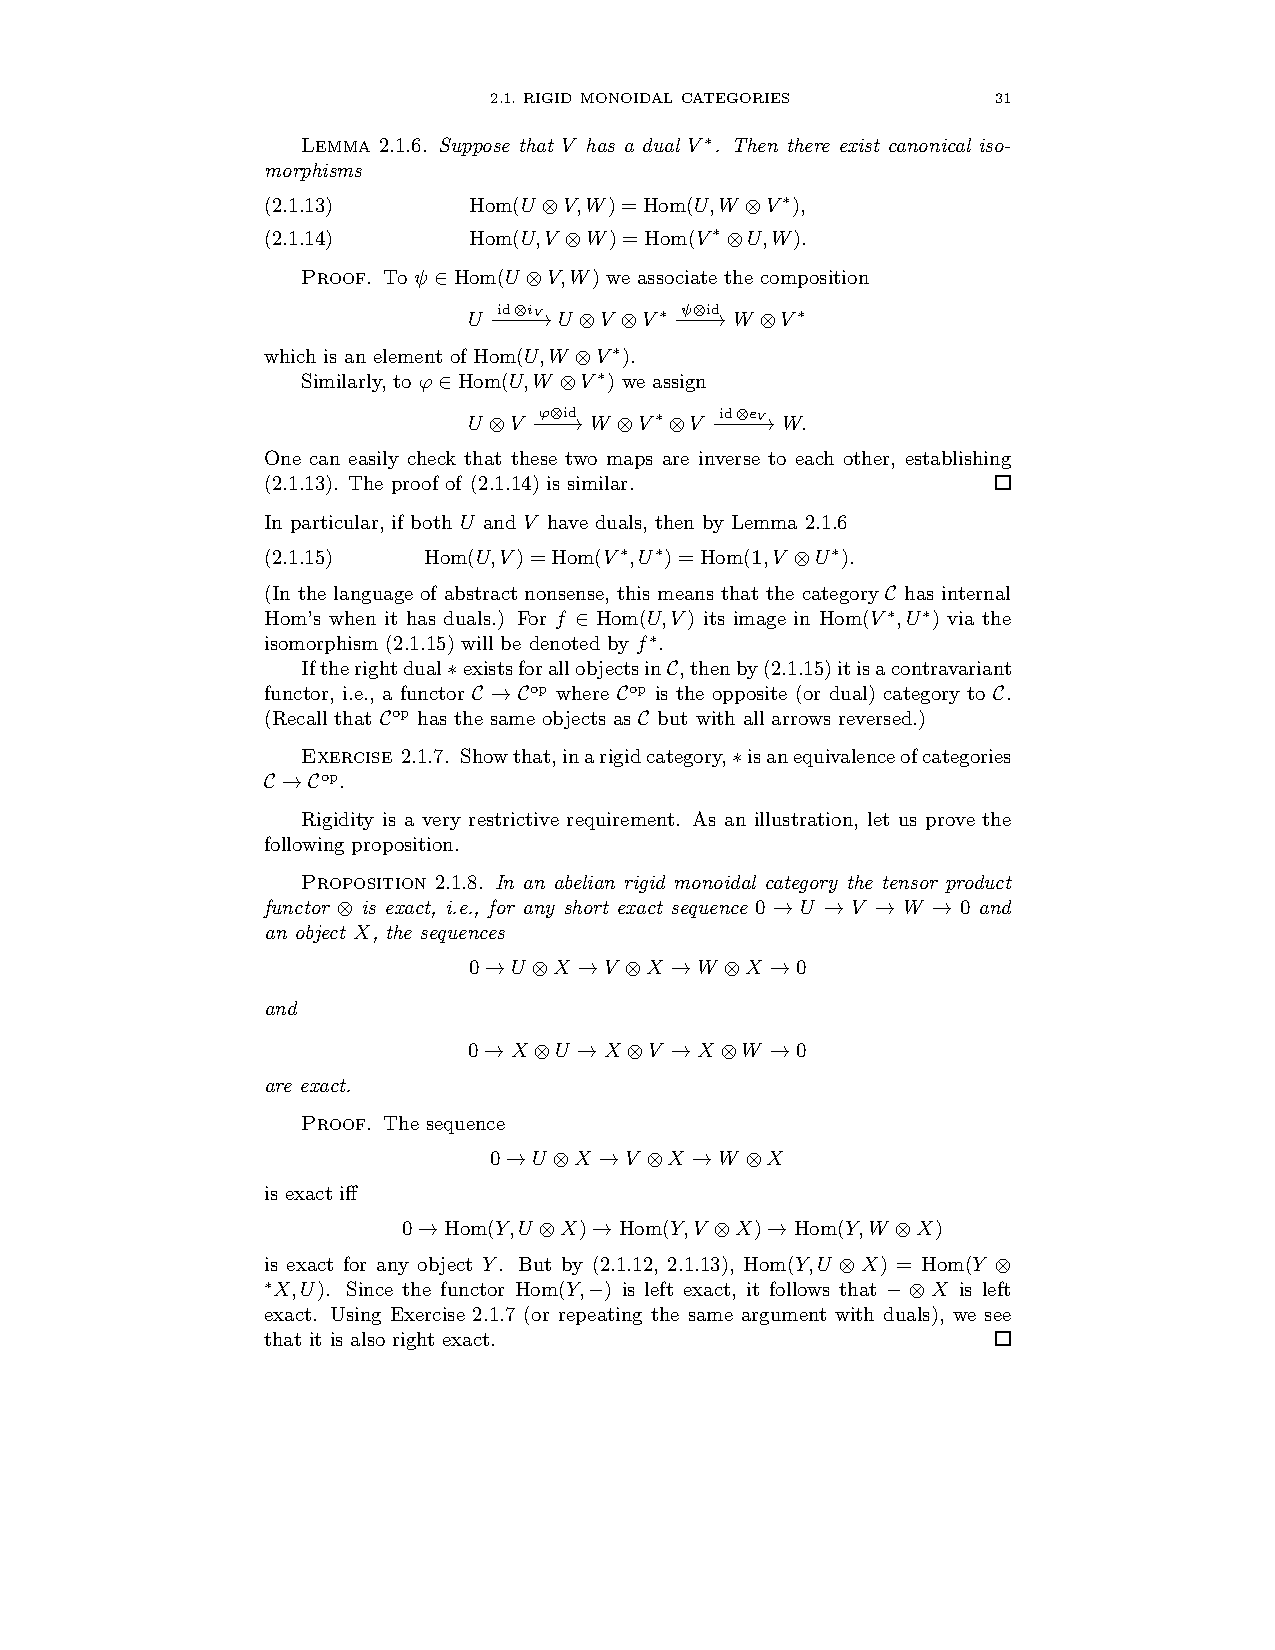
\includepdf[pages=1-last]{BK-p31.pdf}

\end{document}

\newpage
\section{Odds and ends}
\subsection{More on adjoints}
\begin{enumerate}
% \item Give a condition (as weak as you can manage) on a pair of categories $\cC, \cD$, which ensures that a functor $F : \cC \to \cD$ has a left adjoint.
% \item* Consider the forgetful functor from compact Hausdorff spaces into Hausdorff spaces. Show that its left adjoint is Stone-\v{C}ech compactification.
\item Recall the $\cC-\mathsf{Set}$ is the category of functors from $\cC$ to $\mathsf{Set}$. Given a functor $F : \cC \to \cD$, we have the pull-back functor $F^* : \cD-\mathsf{Set} \to \cC-\mathsf{Set}$ given by precomposition by $F$. If $F^*$ has adjoints, we call them the right push-forward $F_*$ and the left pushforward $F_!$ (pronounced usually `$F$-shriek').

(You may like to read \url{https://arxiv.org/abs/1009.1166}.)
\begin{enumerate}
	\item \nn{Calculate some examples.}
	\item Show that the polynomial functors, namely those of the form $F_! G^* H_* : \cE-\mathsf{Set} \to \cB-\mathsf{Set}$ for some diagram $$\cB \xleftarrow{F} \cC \xrightarrow{G} \cD \xleftarrow{H} \cE,$$ are closed under composition. (You may assume that all categories are finitely presented, i.e. the path category of some finite graph modulo finitely many relations. You may like to look at \url{https://ncatlab.org/nlab/show/polynomial+functor}, although as is often the case at the \emph{nLab}, the presentation there is more general than we need.) 
\end{enumerate}

\end{enumerate}



\end{document}

